%% -*- coding: utf-8 -*-
\documentclass[12pt,a4paper]{scrartcl} 
\usepackage[utf8]{inputenc}
\usepackage[english,russian]{babel}
\usepackage{indentfirst}
\usepackage{misccorr}
\usepackage{graphicx}
\usepackage{amsmath}
\usepackage{float}
\begin{document}
\begin{titlepage}
		\begin{center}
			\large
			МИНИСТЕРСТВО НАУКИ И ВЫСШЕГО ОБРАЗОВАНИЯ РОССИЙСКОЙ ФЕДЕРАЦИИ
			
			Федеральное государственное бюджетное образовательное учреждение высшего образования
			
			\textbf{АДЫГЕЙСКИЙ ГОСУДАРСТВЕННЫЙ УНИВЕРСИТЕТ}
			\vspace{0.25cm}
			
			Инженерно-физический факультет
			
			Кафедра автоматизированных систем обработки информации и управления
			\vfill

			\vfill
			
			\textsc{Отчет по практике}\\[5mm]
			
			{\LARGE Программаная реализация численного метода \textit{Сортировки Быстрая и Слиянием. (вариант 4)}}
			\bigskip
			
			2 курс, группа ИВТ АСОИУ
		\end{center}
		\vfill
		
		\newlength{\ML}
		\settowidth{\ML}{«\underline{\hspace{0.7cm}}» \underline{\hspace{2cm}}}
		\hfill\begin{minipage}{0.5\textwidth}
			Выполнил:\\
			\underline{\hspace{\ML}} А.\,Е.~Колесник\\
			«\underline{\hspace{0.7cm}}» \underline{\hspace{2cm}} 2025 г.
		\end{minipage}%
		\bigskip
		
		\hfill\begin{minipage}{0.5\textwidth}
			Руководитель:\\
			\underline{\hspace{\ML}} С.\,В.~Теплоухов\\
			«\underline{\hspace{0.7cm}}» \underline{\hspace{2cm}} 2025 г.
		\end{minipage}%
		\vfill
		
		\begin{center}
			Майкоп, 2025 г.
		\end{center}
	\end{titlepage}
 
\section{Введение.}
\label{sec:intro}
% Что должно быть во введении
Задание:
\begin{description}
    Сортировки Быстрая и Слиянием.
\end{description}
\section{Ход работы}
\label{sec:exp}
\subsection{Код приложения быстрой сортировки}
\label{sec:exp:code}
\begin{verbatim}
#include <iostream>
#include <vector>
#include <math.h>
using namespace std;

int partition(vector<int>& arr, int low, int high) {
    int pivot = arr[high];
    int i = low - 1;
    for (int j = low; j < high; j++) {
        if (arr[j] <= pivot) {
            i++;
            swap(arr[i], arr[j]);
        }
    }
    swap(arr[i + 1], arr[high]);
    return i + 1;
}

void quickSort(vector<int>& arr, int low, int high) {
    if (low < high) {
        int pi = partition(arr, low, high);
        quickSort(arr, low, pi - 1);
        quickSort(arr, pi + 1, high);
    }
}


int main() {
    setlocale(LC_ALL, "RU");
    vector<int> arr = {};
    int n,a;
    cout << "Заполнение массива: \n";
    cout << "Ввод количества значений: \n";
    cin >> n;
    cout << "Ввод значений (целые числа от -100 до 100): \n";
    for (int i = 0;i < n;i++)
    {
        cout << ": ";
        cin >> a;
        if (not(-100 <= a and a <= 100))
        {
            cout << "Введите целое число от -100 до 100\n";
            i--;
        }
        else arr.push_back(a);
    }

    cout << "Исходный массив: ";
    for (int num : arr) cout << num << " ";
    cout << endl;
    quickSort(arr, 0, arr.size() - 1);
    cout << "Отсортированный массив: ";
    for (int num : arr) cout << num << " ";
    cout << endl;
    return 0;
}
\end{verbatim}

\subsection{Код приложения сортировки слиянием}
\label{sec:exp:code}
\begin{verbatim}
#include <iostream>
#include <vector>
#include <math.h>
using namespace std;

void merge(vector<int>& arr, int left, int mid, int right) {
    int n1 = mid - left + 1;
    int n2 = right - mid;

    vector<int> L(n1), R(n2);

    for (int i = 0; i < n1; i++)
        L[i] = arr[left + i];
    for (int j = 0; j < n2; j++)
        R[j] = arr[mid + 1 + j];

    int i = 0;
    int j = 0;
    int k = left;

    while (i < n1 && j < n2) {
        if (L[i] <= R[j]) {
            arr[k] = L[i];
            i++;
        }
        else {
            arr[k] = R[j];
            j++;
        }
        k++;
    }

    while (i < n1) {
        arr[k] = L[i];
        i++;
        k++;
    }

    while (j < n2) {
        arr[k] = R[j];
        j++;
        k++;
    }
}

void mergeSort(vector<int>& arr, int left, int right) {
    if (left < right) {
        int mid = left + (right - left) / 2;

        mergeSort(arr, left, mid);
        mergeSort(arr, mid + 1, right);

        merge(arr, left, mid, right);
    }
}

int main() {
    setlocale(LC_ALL, "RU");
    vector<int> arr = {};
    int n, a;
    cout << "Заполнение массива: \n";
    cout << "Ввод количества значений: \n";
    cin >> n;
    cout << "Ввод значений (целые числа от -100 до 100): \n";
    for (int i = 0;i < n;i++)
    {
        cout << ": ";
        cin >> a;
        if (not(-100 <= a and a <= 100))
        {
            cout << "Введите целое число от -100 до 100\n";
            i--;
        }
        else arr.push_back(a);
    }

    cout << "Исходный массив: ";
    for (int num : arr) cout << num << " ";
    cout << endl;

    mergeSort(arr, 0, arr.size() - 1);

    cout << "Отсортированный массив: ";
    for (int num : arr) cout << num << " ";
    cout << endl;
    return 0;
}
\end{verbatim}
\section{Примеры работы программ:}
\subsection{Быстрая сортировка: }
\label{sec:pictures1}
\begin{figure}[H]
	\centering
	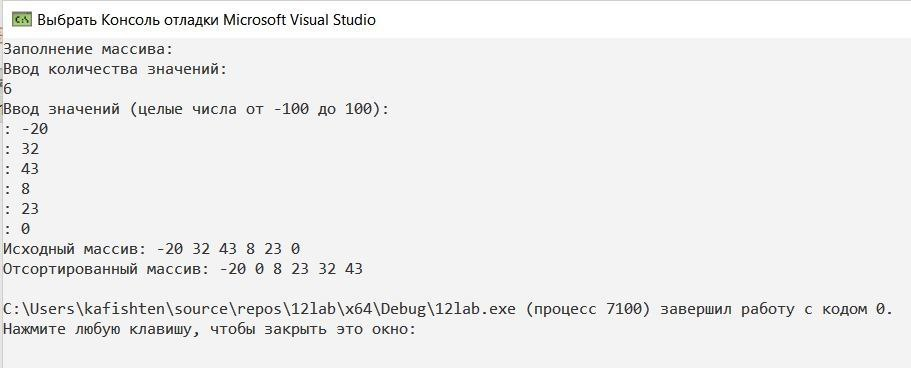
\includegraphics[width=0.9\textwidth]{1.jpg}
	\caption{Пример работы программы быстрой сортировки с ручным вводом значений}\label{fig:par}
\end{figure}

\subsection{Сортировка слиянием: }
\begin{figure}[H]
  \centering
  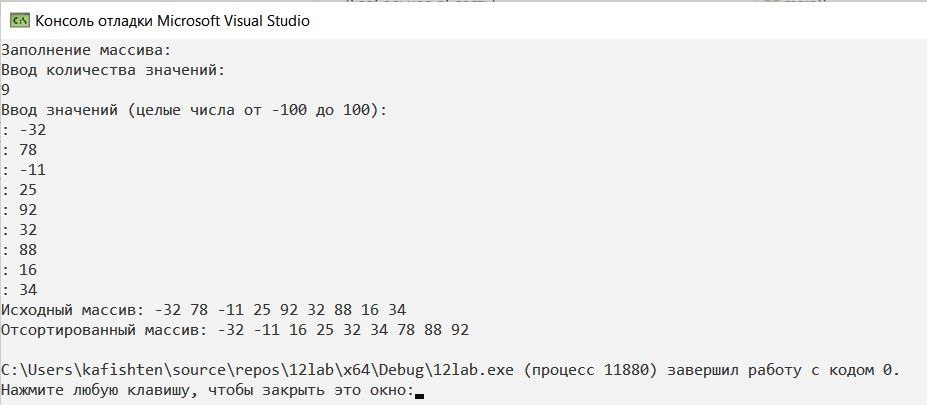
\includegraphics[width=0.9\textwidth]{2.jpg}
  \caption{Пример работы программы сортировки слиянием с ручным вводом значений.}
  \label{fig:par2}
\end{figure}





\begin{thebibliography}{9}
\label{sec:biblio}
\bibitem{Lvovsky-2003}Львовский С.М. Набор и верстка в системе \LaTeX{}. \newblock --- 3-е издание, исправленное и дополненное, 2003 г.
\bibitem{Voroncov-2005}Воронцов К.В. \LaTeX{} в примерах. 2005 г.
\end{thebibliography}
\end{document}
